\chapter{Introduction}
\label{chap:intro}
Probabilities describe degrees of belief, and probabilistic inference describes rational reasoning under uncertainty. Undoubtedly, probabilistic models have exploded onto all the sciences of inference under uncertainty: machine learning, information retrieval, applied statistics and artificial intelligence. However, it's not easy for common programmers to describe the probabilistic models and encode the probabilistic inference. Especially when the probabilistic models become complicated, the complexity to describe them and to perform inference will also be raised. Just as programming beyond the simplest algorithms requires tools for abstraction and composition, complex probabilistic modeling requires new progress in model representation - probabilistic programming languages. Probabilistic programming languages are in the spotlight, which provide compositional means for describing complex probability distributions and performing efficient probabilistic inference. ~\cite{goodman}.

The goal of probabilistic programming is to enable probabilistic modeling and machine learning to be accessible to the working programmer, who has sufficient domain expertise, but perhaps not enough expertise in probability theory or machine learning. We wish to hide the details of inference inside the compiler and runtime, and enable the programmers to express models using their domain expertise and dramatically increase the number of programmers who can benefit from probabilistic modeling. In Probabilistic programming, modeling and inference have been disentangled.

In this chapter, the background information of probabilistic programming will be introduced. In section ~\ref{sec:pp}, we will illustrate what is probabilistic programs and will give some simple examples. In section ~\ref{sec:pgm}, we will introduce probabilistic graphical models, especially the relationships between probabilistic programs and other probabilistic models that readers may have encountered before. Two kinds of probabilistic graphical models will be discussed: Bayesian networks and Markov networks. In section ~\ref{sec:inferintro}, we will elaborate on the probabilistic inference technologies and show some examples of probabilistic inference problems. In section ~\ref{sec:language}, the formalized probabilistic programming language will be defined and the difference between common programming languages and probabilistic programming languages according to syntax and semantics will be illustrated. 

\section{Probabilistic Programs}
\label{sec:pp}
\textit{Probabilistic programs} are ``usual" programs (written in languages like C, Java, Ocaml or Lisp) with two additional constructs: (1) the ability to draw values at random from distributions (like gaussian, gamma, etc.), and (2) the ability to condition values of variables in a program via observe statements (which can incorporate data from real world observations into a probabilistic program). ~\cite{gordon2014}. A variety of probabilistic programming languages and systems have been proposed, including BUGS ~\cite{bugs}, Church ~\cite{church}, FACTORIE ~\cite{factorie}, Infer.NET ~\cite{infernet}, Dimple ~\cite{dimple}, etc. However, unlike usual programs which are written for the purpose of being executed, the purpose of a probabilistic program is to implicitly specify a probability distribution. 

We introduce the syntax and semantics of probabilistic programs using two simple probabilistic programs from Figure ~\ref{fig:pp_simple_eg}. This is an example written in \textbf{Probabilistic C}. Drawing from a Bernoulli distribution with mean 0.5 can be seen as tossing fair coins. The program in the top, Example $1(a)$, tosses two fair coins, and respectively assigns the outcomes of these coin tosses to the Boolean variables $c_1$ and $c_2$, and returns $(c_1, c_2)$. The semantics of this program is the expectation of its return value. In this case, the return value will be $(1/2, 1/2)$. Since we have that 
\begin{align*}
  P( c_1 = false, c_2 = false) &=\\
  P(c_1=false, c_2=true) &= \\
  P(c_1=true, c_2=false) &= \\
  P(c_1=true, c_2=true) &= 1/4
\end{align*}
we have that the expectation on the return value is given by 
\begin{align*}
  1/4 \times (0, 0) + 1/4 \times (0, 1) + 1/4 \times (1, 0) + 1/4 \times (1, 1) = (1/2, 1/2)
\end{align*}
where we treated true as $1$ and false as $0$.

The program in Example $1(b)$ is slightly different from Example $1(a)$. It has an observe statement $observe(c_1 \| c_2)$ before returning the value of $(c_1,c_2)$. The observe statement blocks runs which do not satisfy the boolean expression $c_1 \| c_2$ and does not permit those executions to happen. Executions that satisfy $c_1 \| c_2$ are permitted to happen. It is sort of a condition that the varibales need to meet. Thus the semantics of the program is the expected return value conditioned by $(c_1 \| c_2)$, the permitted executions. Since conditioning by permitted executions yields
\begin{align*}
  P(c_1=false,c_2=false) &= 0 \\
  P(c1=false,c2=true) &= \\
  P(c1=true,c2=false) &= \\
  P(c1=true,c2=true) &= 1/3
\end{align*}
we have that the different expected return value which is 
\begin{align*}
  0 \times (0,0) + 1/3 \times (0,1) + 1/3 \times (1,0) + 1/3 \times (1,1) = (2/3,2/3).
\end{align*}

\begin{figure}
    \centering
    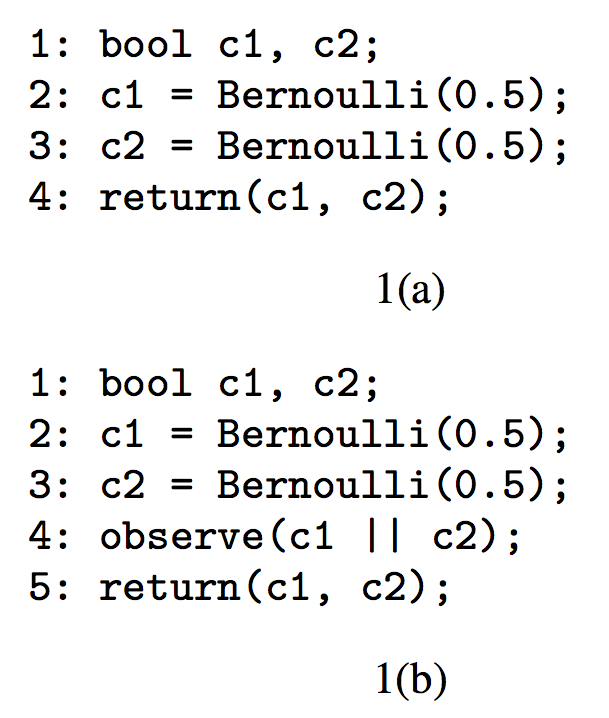
\includegraphics[width=0.4\textwidth]{figures/pp_simple_eg.png}
    \caption{Simple probabilistic programs}
    \label{fig:pp_simple_eg}
\end{figure}

Another example of the probabilistic programs is for Latent Dirichlet Allocation (LDA), which can be seen in Figure ~\ref{fig:lda}. In the LDA example, the words in blue represent probabilistic distributions with the arguments as parameters of the distributions. Each time a value can be sampled from the specified probabilistic distributions, such as \textbf{dirichlet}, \textbf{multinomial}, \textbf{gaussian}, etc. The trace of the sampled value meet the requirement of the corresponding probabilistic distribution. Compared with the LDA program coding in some comman languages like C, Python, or Matlab in hundreds of lines, which contains both of the modeling code and inference code, programming in probabilistic programming language is a big relief for programmers and much easier to read the program.

\begin{figure}
    \centering
    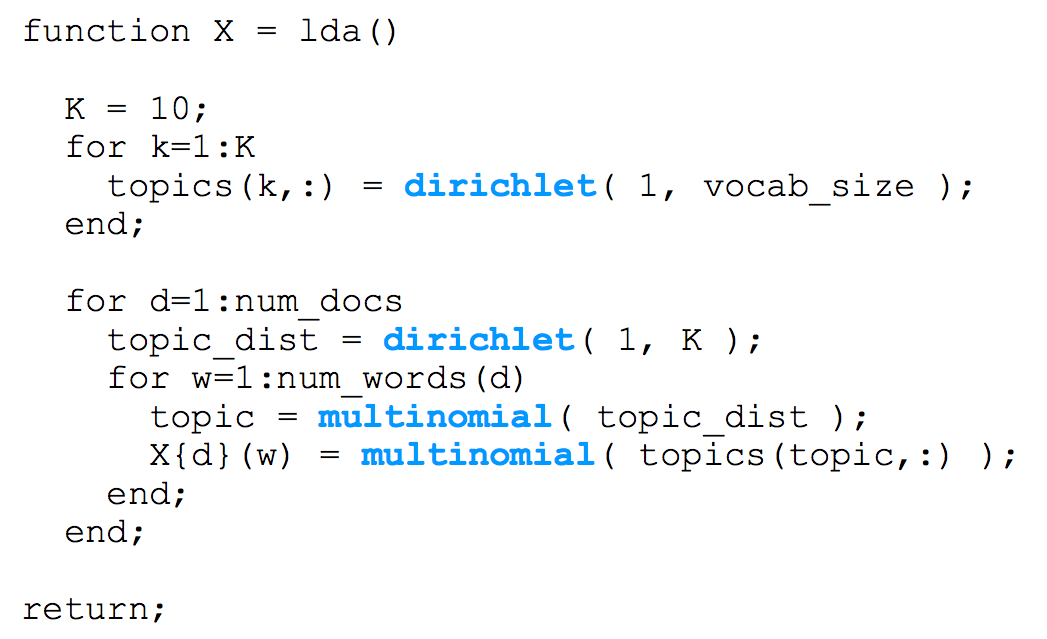
\includegraphics[width=0.9\textwidth]{figures/lda_eg.png}
    \caption{Probabilistic program example: LDA.}
    \label{fig:lda}
\end{figure}


\section{Probabilistic Graphical Model}
\label{sec:pgm}
Probabilistic programs can be used to represent probabilistic graphical models ~\cite{pgm}, which use graphs to denote conditional dependences between random variables.

\textit{Probabilistic graphical models(PGM)} use a graph based representation as the basis for compactly encoding a complex distribution over a high-dimensional space. In the graphical representation illustrated in Figure ~\ref{fig:pgm}, the nodes (or ovals) correspond to the variables in the domain, and the edges correspond to direct probabilistic interactions between them. For example, in Figure ~\ref{fig:pgm}, the top of (a) illustrates one possible graph structure for a patient example, where \texttt{Flu} depends on \texttt{Season} and \texttt{Congestion} depends on \texttt{Hayfever}. In this graph, we can see that there is no direct edge between \texttt{Muscle Pain} and \texttt{Season}, but both interact directly with Flu. There are two perspectives that one can use to interpret the structure of this graph. From one perspective, the graph is a compact representation of a set of independencies that hold in the distribution; these properties take the form $X$ is independent of $Y$ given $Z$, denoted $(X \bot Y | Z)$, for some subsets of variables $X, Y ,Z$. In this example, the distribution satisfies the conditional independence $(Congestion \bot Season | Flu, Hayfever)$. This statement asserts that

\begin{align*}
P(Congestion | Flu, Hayfever, Season) = P(Congestion | Flu, Hayfever);
\end{align*}

that is, if we are interested in the distribution over the patient having congestion, and we know whether he has the flu and whether he has hayfever, the season is no longer informative. But this assertion does not imply that \texttt{Season} is independent of \texttt{Congestion}. Figure ~\ref{fig:pgm}a (middle) shows the set of independence assumptions associated with the graph in Figure ~\ref{fig:pgm}a (top).

The other perspective is that the graph model describes a skeleton for compactly representing a high dimensional factor graph. Rather than encode the probability of every possible assignment to factor all of the variables in our domain, we can ``break up" the distribution into smaller factors, each over a much smaller space of possibilities. We can then define the overall joint distribution as a product of these factors. For example, Figure ~\ref{fig:pgm}a (bottom) shows the factorization of the distribution associated with the graph in Figure ~\ref{fig:pgm}a (top). It asserts, for example, that the probability of the event “spring, no flu, hayfever, sinus congestion, muscle pain” can be obtained by multiplying five numbers:
\begin{align*}
  P&(Season = spring)\\
  P&(Flu = false | Season = spring)\\
  P&(Hayfever = true | Season = spring)\\
  P&(Congestion = true | Hayfever = true,Flu = false)\\
  P&(Muscle Pain = true | Flu = false)
\end{align*}
The graph structure defines the factorization of a distribution $P$ associated with it - the set of factors and the variables that they encompass.

We describe two families of graphical representations of distributions. One, called Bayesian networks, uses a directed graph (where the edges have a source and a target), as shown in Figure ~\ref{fig:pgm}a (top). The second, called Markov networks, uses an undirected graph, as illustrated in Figure ~\ref{fig:pgm}b (top). It can be viewed as defining a set of independence assertions (Figure ~\ref{fig:pgm}b (middle) or as encoding a compact factorization of the distribution as showed in Figure ~\ref{fig:pgm}b (bottom). Both representations provide the duality of independencies and factorization, but they differ in the set of independencies they can encode and in the factorization of the distribution that they induce. In this paper we will focus more on Bayesian networks.

\begin{figure}
    \centering
    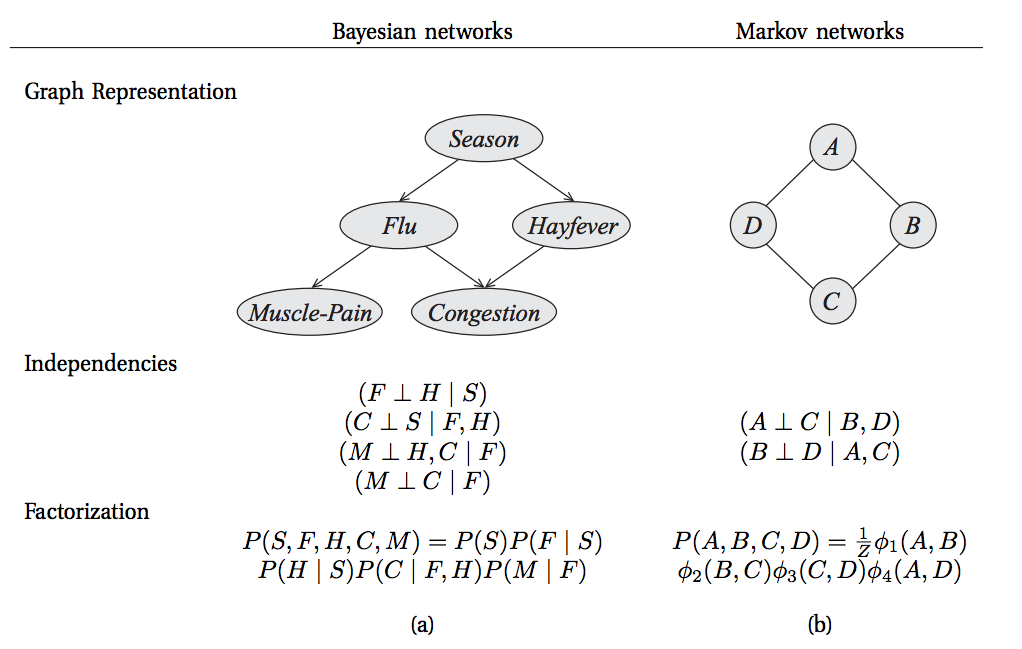
\includegraphics[width=\textwidth]{figures/pgm.png}
    \caption{Probabilistic graphical models in different perspectives: the graphical representation (top); the independencies induced by the graph structure (middle); the factorization induced by the graph structure (bottom). (a) A sample Bayesian network. (b) A sample Markov network.}
    \label{fig:pgm}
\end{figure}


\subsection{Bayesian Networks}
A Bayesian network structure is a directed, acyclic graph $G$, where each vertex $s$ of $G$ is interpreted as a random variable $X_s$ (with unspecified distribution) ~\cite{heckerman}.
A Bayesian network $(G, P)$ consists of
\begin{itemize}
  \item a BN structure G and
  \item a set of conditional probability distributions (CPDs) $P(X_s | Pa_{X_s})$, where $Pa_{X_s}$ are the parents of node $X_s$ such that 
  \item $(G, P)$ defines a joint distribution
  \begin{align*}
    P(X_i, \dots, X_n) = \prod_i P(X_i | Pa_{X_i})
  \end{align*}
\end{itemize}
There are three main inference tasks for Bayesian networks.

\subsubsection{Inferring Unobserved Variables}
Since a Bayesian network is a complete model for the variables and their relationships, it can be used to answer probabilistic queries about them. For example, the network can be used to find out updated knowledge of the state of a subset of variables when other variables (the evidence variables) are observed. This process of computing the posterior distribution of variables given evidence is called probabilistic inference. The posterior gives a universal sufficient statistic for detection applications, when one wants to choose values for the variable subset which minimize some expected loss function, for instance the probability of decision error. A Bayesian network can thus be considered a mechanism for automatically applying Bayes' theorem to complex problems.


\subsubsection{Parameter Learning}
In order to fully specify the Bayesian network and thus fully represent the joint probability distribution, it is necessary to specify for each node $X$ the probability distribution for $X$ conditional upon $X's$ parents. The distribution of $X$ conditional upon its parents may have any form. It is common to work with discrete or Gaussian distributions since that simplifies calculations. Sometimes only constraints on a distribution are known; one can then use the principle of maximum entropy to determine a single distribution, the one with the greatest entropy given the constraints. (Analogously, in the specific context of a dynamic Bayesian network, one commonly specifies the conditional distribution for the hidden state's temporal evolution to maximize the entropy rate of the implied stochastic process.)

Often these conditional distributions include parameters which are unknown and must be estimated from data, sometimes using the maximum likelihood approach. Direct maximization of the likelihood (or of the posterior probability) is often complex when there are unobserved variables. A classical approach to this problem is the expectation-maximization algorithm which alternates computing expected values of the unobserved variables conditional on observed data, with maximizing the complete likelihood (or posterior) assuming that previously computed expected values are correct. Under mild regularity conditions this process converges on maximum likelihood (or maximum posterior) values for parameters.

A more fully Bayesian approach to parameters is to treat parameters as additional unobserved variables and to compute a full posterior distribution over all nodes conditional upon observed data, then to integrate out the parameters. This approach can be expensive and lead to large dimension models, so in practice classical parameter-setting approaches are more common.

\subsubsection{Structure Learning}
In the simplest case, a Bayesian network is specified by an expert and is then used to perform inference. In other applications the task of defining the network is too complex for humans. In this case the network structure and the parameters of the local distributions must be learned from data.

Automatically learning the graph structure of a Bayesian network is a challenge pursued within machine learning. The basic idea goes back to a recovery algorithm developed by ~\cite{recovery} and rests on the distinction between the three possible types of adjacent triplets allowed in a directed acyclic graph (DAG):
\begin{align*}
  X \rightarrow Y \rightarrow Z
  X \leftarrow Y \rightarrow Z
  X \rightarrow Y \leftarrow Z
\end{align*}

Type 1 and type 2 represent the same dependencies (X and Z are independent given Y) and are, therefore, indistinguishable. Type 3, however, can be uniquely identified, since X and Z are marginally independent and all other pairs are dependent. Thus, while the skeletons (the graphs stripped of arrows) of these three triplets are identical, the directionality of the arrows is partially identifiable. The same distinction applies when X and Z have common parents, except that one must first condition on those parents. Algorithms have been developed to systematically determine the skeleton of the underlying graph and, then, orient all arrows whose directionality is dictated by the conditional independencies observed.~\cite{causality}

An alternative method of structural learning uses optimization based search. It requires a scoring function and a search strategy. A common scoring function is posterior probability of the structure given the training data. The time requirement of an exhaustive search returning a structure that maximizes the score is superexponential in the number of variables. A local search strategy makes incremental changes aimed at improving the score of the structure. A global search algorithm like Markov chain Monte Carlo can avoid getting trapped in local minima. ~\cite{friedman} talk about using mutual information between variables and finding a structure that maximizes this. They do this by restricting the parent candidate set to k nodes and exhaustively searching therein.

\subsection{Markov Networks}
\textit{Markov network}, or \textit{Markov random field} is a set of random variables having a Markov property described by an undirected graph. A Markov random field is similar to a Bayesian network in its representation of dependencies; the differences being that Bayesian networks are directed and acyclic, whereas Markov networks are undirected and may be cyclic. Thus, a Markov network can represent certain dependencies that a Bayesian network cannot (such as cyclic dependencies); on the other hand, it can't represent certain dependencies that a Bayesian network can (such as induced dependencies).~\cite{markov}.\\

In our framework, the language targets to describe Bayesian networks and solves the query of inferring unobserved variables by probabilistic inference.

\section{Probabilistic Inference}
\label{sec:inferintro}
\textit{Probabilistic inference} is the problem of computing an explicit representation of the probability distribution implicitly specified by a probabilistic program. If the probability distribution is over a large number of variables, an explicit representation of the joint probability distribution may be both difficult to obtain efficiently, and unnecessary in the context of specific application contexts. For example, we may want to compute the expected value of some function $f$ with respect to the distribution (which may be more efficient to calculate without representing the entire joint distribution). Alternatively, we may want to calculate the most likely value of the variables, which is the mode of the distribution. Or we may want to simply draw a set of samples from the distribution, to test some other system which expects inputs to follow the modeled distribution. ~\cite{gordon2014}.

\begin{figure}
    \centering
    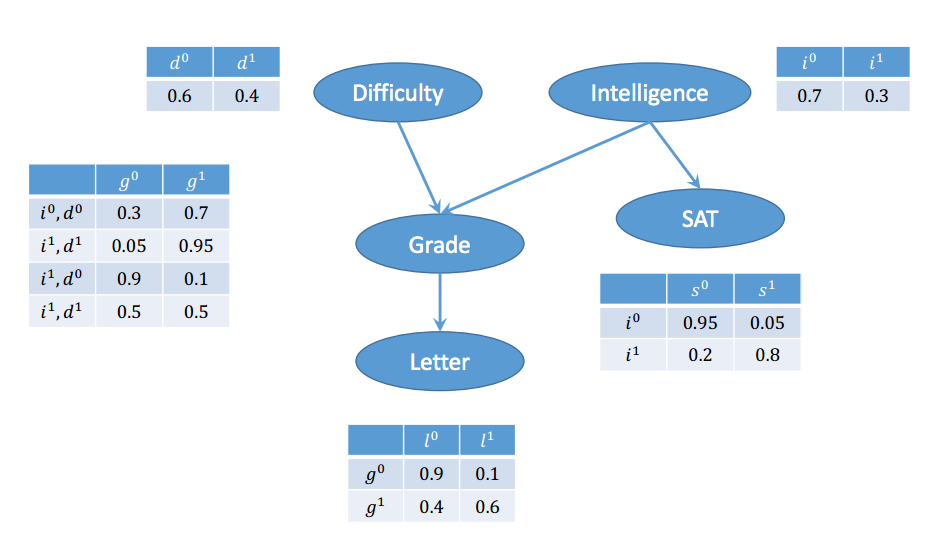
\includegraphics[width=0.9\textwidth]{figures/inference.png}
    \caption{A student example to show probabilistic inference.}
    \label{fig:infer_eg}
\end{figure}

Figure ~\ref{fig:infer_eg}. gives an example of inference problem. The variable Difficulty describes the difficulty of the courses with probability $0.6$ to be not hard, namely $d_0$, and probability $0.4$ to be $d_1$. Other variables share the similar meaning with Difficulty. If we want to know the probability of the student can get $Letter = l_1$ under the condition his grade $Grade = g_1$, then this is an inference problem with the formal representation $P (L = l_1 | G = g_1)$. Also, if we want to know the probability of the student getting $Grade = g_1$ under he/she has already get the $Letter = l_1$, which is backward compared with the previous conditional probability, this is also the problem of probabilistic inference with the formal representation $P (G = g_1 | L = l_1)$.

Threre are two kinds of inference technologies, exact inference and approximate inference. The most common exact inference methods are: variable elimination, which eliminates (by integration or summation) the non-observed non-query variables one by one by distributing the sum over the product; clique tree propagation, which caches the computation so that many variables can be queried at one time and new evidence can be propagated quickly; and recursive conditioning and AND/OR search, which allow for a space-time tradeoff and match the efficiency of variable elimination when enough space is used. All of these methods have complexity that is exponential in the network's treewidth. The most common approximate inference algorithms are importance sampling, stochastic Markov chain Monte Carlo(MCMC) simulation ~\cite{mcmc}, mini-bucket elimination, loopy belief propagation, generalized belief propagation, and variational methods.

In this paper, we leveraged approximate inference technologies including rejection sampling ~\cite{reject} and Metroplis-Hastings algorithm ~\cite{mh}. More details can be found in Chapter \ref{chap:approach}.

\section{Probabilistic Programming Language}
\label{sec:language}
\textit{Probabilistic Programming Languages(PPL)} extend a well-specified deterministic programming language with primitive constructs for random choice. Just as with deterministic programming languages, there are probabilistic languages in the imperative, functional, and logical paradigms. We will take one of the probabilistic programming language \textbf{Probabilistic C} ~\cite{probc} as example, which is a C-like imperative programming language with two additional statements:
\begin{enumerate}
  \item The probabilistic assignment $"x \sim Dist(\bar{\theta})"$ draws a sample from a distribution Dist with a vector of parameters $\bar{\theta}$, and assigns it to the variable $x$. For instance, the statement $"x \sim Gaussian(\mu, \sigma)"$ draws a value from a Gaussian distribution with mean $\mu$ and standard deviation $\sigma$, and assigns it to the variable $x$.
  \item The observe statement $"observe(\varphi)"$ conditions a distribution with respect to a predicate or condition $\varphi$ that is defined over the variables in the program. In particular, every valid execution of the program must satisfy all conditions in observe statements that occur along the execution.
\end{enumerate}

\begin{figure}
    \centering
    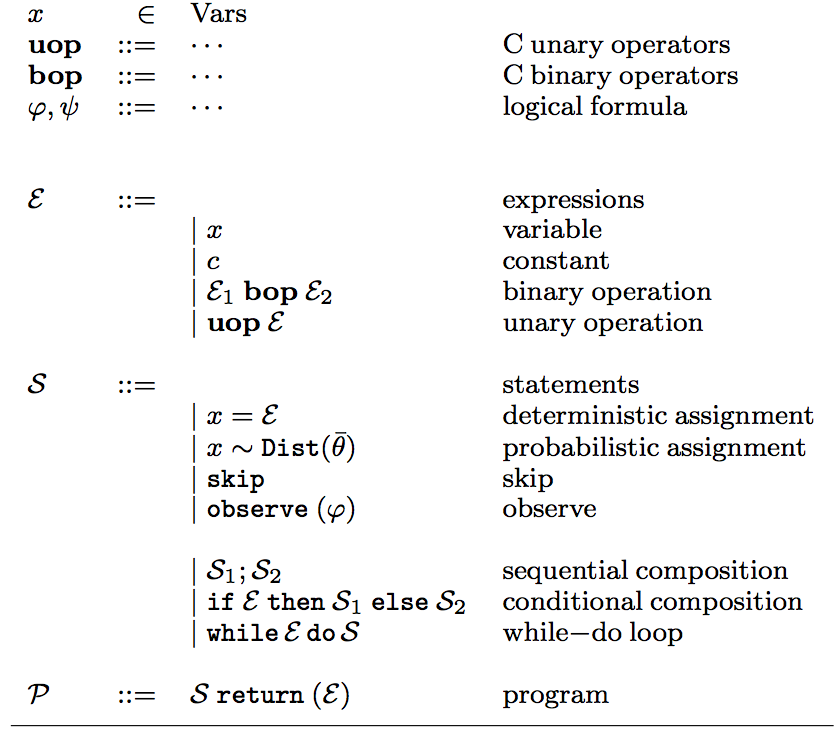
\includegraphics[width=0.6\textwidth]{figures/prob_syntax.png}
    \caption{Syntax of PROB}
    \label{fig:prob_syntax}
\end{figure}
The syntax of \textbf{Probabilistic C} is formally described in Figure ~\ref{fig:prob_syntax}. A program consists of a statement and a return expression. Variables have base types such as int, bool, float and double. Expressions include variables, constants, binary and unary operations.

Statements include primitive statements (deterministic assignment, probabilistic assignment, observe, skip ) and composite statements (sequential composition, conditionals and loops). Features such as arrays, pointers, structures and function calls can be included in the language, and their treatment does not introduce any additional challenges due to probabilistic semantics. Therefore, we omit these features, and focus on a core language.\\

In summary, probabilistic graphical models are the representations of the structure of probabilistic distributions. One can derive the explicit representation of probability distribution by probabilistic inference. Probabilistic programming language can describe probabilistic graphical models and query some conditional probability or joint probability. So probabilistic programs have two extra feature than usual programs: 
\begin{enumerate}
  \item Draw samples from probabilistic distribution
  \item Query some probabilisty.
\end{enumerate}

In Chapter ~\ref{chap:related}, the related work will be introduced including the state of the art probabilistic programming languages and systems. In Chapter ~\ref{chap:approach}, we will elaborate on the approach of the design and implementation of the portable probabilistic programming framework. More specifically, the syntax of the language is illustrated in section ~\ref{sec:syntax} and the implementation of the probabilistic library is showed in section ~\ref{sec:distr}. The algorithms of probabilistic inference and the implementation of the inference engine are elaborated in section ~\ref{sec:infer}. And the implementation of the APIs for other common programming languages is illustrated in section ~\ref{sec:api}. In Chapter ~\ref{chap:eval}, the examples of using our framework as well as the benchmarks will be showed. In Chapter ~\ref{chap:conclusion}, we will conclude our work and the future work that can be done based our framework. 

